\section{Plant papers}
\subsection{Ye (2013) Evolutionary analyses of non-family genes in plants}

    Citation \cite{ye_evolutionary_2013}

    The paper isn't focused at all on orphans. The main interest is (as the
    title suggests) non-family genes.

    \begin{description} \item[NF] non-family (1-2 per genome) \item[LF]
            low-copy family (3-10 per genome) \item[HF] high-copy family
                (>10 per genome \end{description}

    Cluster analysis on 14 plant genomes. Identifies rough strata. Counts
    strata-specific non-family (NF) genes. Arabidopsis thaliana is the only
    Brassicacea member.

    \begin{figure}[h!] \centering 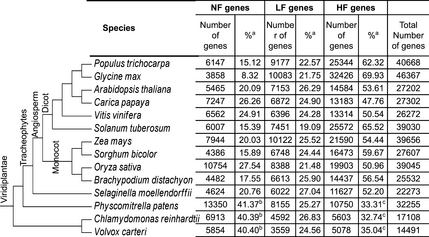
\includegraphics{ye_nonfamily-fig1}
        \caption{ ${}^b$ Lower plants have significantly ($P < 0.01$,
        Chi-square) higher proportion of NF genes than higher plants.
        ${}^c$ Lower plants have significantly ($P < 0.01$, Chi-square)
        lower proportion of HF genes than higher plants } \end{figure}

    \begin{figure}[h!] \centering 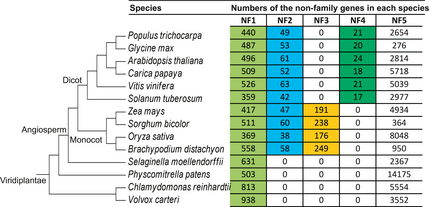
\includegraphics{ye_nonfamily-fig3}
        \caption{ Distribution of non-family (NF; 1 or 2 copies) genes
            among different phylogenetic groups. NF1 gene group contains NF
            genes having homologues in all the 14 species; NF2 contains NF
            genes having homologues in all and only the 10 angiosperm
            species; NF3 contains NF genes having homologues in all and
            only the four monocot species; NF4 contains NF genes having
            homologues in all and only the six dicot species; and NF5
            contains species-specific NF genes. The numbers of genes in
        each species were normalized based on Glycine, which has the
    highest number of genes among the 14 species studied.  } \end{figure}

    \begin{figure}[h!] \centering 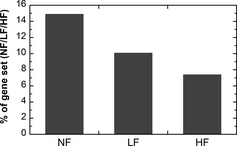
\includegraphics{ye_nonfamily-fig8}
        \caption{ Hub genes in non-family (NF; 1 or 2 copies),
            low-copy-number family (LF; 3-10 copies) and high-copy-number
            family (HF; $>$10 copies) sets. Hubs were defined here as the
            top 10\% most connected nodes in the Arabidopsis
        protein-protein interaction network } \end{figure} \FloatBarrier

\subsection{Guo (2013) Gene family evolution in green plants with emphasis
    on the origination and evolution of \textit{Arabidopsis thaliana}
genes}

\subsection{Freeling (2012) Fractionation mutagenesis and similar consequences
    of mechanisms removing dispensable or less-expressed {DNA} in plants}

    Citation \cite{freeling_fractionation_2012}

    Junk hangs out for millions of years in mammals, but flowering plants take
    out the garbage. For example, all 200 dead genes in the human lineage
    remain as pseudogenes \cite{schrider_all_2009}. However in plants maize
    \cite{woodhouse_following_2010} and Arabidopsis
    \cite{thomas_following_2006} extremely rapid loss of duplicated genes were
    found to follow tetraploidy events. The main mechanism is intra-chromosomal
    or illgenimate recombination \cite{woodhouse_following_2010}.

\subsection{Wang (2010) Evolutionary Transients in the Rice Transcriptome}

    Citation \cite{wang_evolutionary_2010}

    The tail of the degenerate twin

    ``In the canonical version of evolution by gene duplication, one copy
    is kept unaltered while the other is free to evolve. This process of
    evolutionary experimentation can persist for millions of years. Since
    it is so short lived in comparison to the lifetime of the core genes
    that make up the majority of most genomes, a substantial fraction of
    the genome and the transcriptome may—in principle—be attributable to
    what we will refer to as “evolutionary transients”, referring here to
    both the process and the genes that have gone or are undergoing this
    process. Using the rice gene set as a test case, we argue that this
    phenomenon goes a long way towards explaining why there are so many
    more rice genes than Arabidopsis genes, and why most excess rice genes
    show low similarity to eudicots.'' abstract, pp. 1

    
\subsection{Luhua (2008) Enhanced Tolerance to Oxidative Stress in Transgenic
Arabidopsis Plants Expressing Proteins of Unknown Function}

Citation \cite{luhua_enhanced_2008}

The study is focused on POFs (proteins of obscure function) rather than
orphans. But it identifies the rough strata of all of the POFs. This paper
is particularly important because it contains experimental verification of
several functional orphans.

Procedure: Identified 41 POFs that respond to oxidative stress and
expressed them constitutively in transgenic A. thaliana lines.

``We found that more than 70\% of the expressed unknown proteins conferred
tolerance to oxidative stress. In contrast, the majority of expressed
unknowns (.90\%) did not confer tolerance to the other stresses tested, and
approximately 50\% of the expressed un- known proteins rendered plants more
susceptible to osmotic or salinity stress'', pp. 2

At-specific loci:

\begin{description}

    \item[AT1G21520] l=66; BLAST(nr) genus-specific 

    \item[AT1G50290] l=134; BLAST(nr) species-specific (e-0.004 to lyrata)

    \item[AT1G64360] l=85; BLAST(nr) Camelineae-specific (strong match to
        Capsella). $~$6-fold upregulated under osmotic stress.
    
    \item[AT2G41650] l=66; BLAST(nr) species-specific. $~$2-fold
        upregulated under oxidative stress.
        
\end{description}

Brassica-specific loci: AT2G22080, AT5G18040

\begin{description}

    \item[AT2G22080] l=177; BLAST(nr) Zinc-finger domain. $~$15-fold
        upregulated under oxidative stress.

    \item[AT5G18040] l=; BLAST(nr)

\end{description}

Identifies 2 Arabidopsis specific and 1 Brassica-specific oxidative stress
tolerance enhancing genes.

\subsection{Armisen (2008) Unique genes in plants: specificities and
conserved features throughout evolution}

    Citation \cite{armisen_unique_2008}

    Based only on Arabidopsis and Oryza

    Focused on unique (as in single-family) genes, not specfically orphans.
    Orphans are genes with no orthologs, unique genes are those with no
    paralogs.

    ``Many of the A. thaliana and O. sativa unique genes are conserved in
    plants for which the ancestor diverged at least 725 million years ago
    (MYA). Half of these genes are also present in other eukaryotic and/or
    prokaryotic species. Thus, our results indicate that (i) a strong
    negative selection pressure has conserved a number of genes as unique
    in genomes throughout evolution, (ii) most unique genes are subjected
    to a low divergence rate, (iii) they have some features observed in
    housekeeping genes but for most of them there is no functional
    annotation and (iv) they may have an ancient origin involving a
    possible gene transfer from ancestral chloroplasts or bacteria to the
    plant nucleus.'' pp. 1

\subsection{Castellana (2008) Discovery and revision of Arabidopsis genes by proteogenomics}

    All based on TAIR7, TAIR8 does not incorporate their work and only 3\% of
    the novel genes Castellana finds are added to TAIR8. TAIR9 incorporated
    Castellana's results \cite{lamesch_arabidopsis_2011}.

    Castellana says genomics and proteomics people should be friends.

    Citation \cite{castellana_discovery_2008}

    ``Gene annotation underpins genome science. Most often protein coding
    sequence is inferred from the genome based on transcript evidence and
    computational predictions. While generally correct, gene models suffer from
    errors in reading frame, exon border definition, and exon identification.
    To ascertain the error rate of Arabidopsis thaliana gene models, we
    isolated proteins from a sample of Arabidopsis tissues and determined the
    amino acid sequences of 144,079 distinct peptides by tandem mass spectrom-
    etry. The peptides corresponded to 1 or more of 3 different translations of
    the genome: a 6-frame translation, an exon splice- graph, and the currently
    annotated proteome. The majority of the peptides (126,055) resided in
    existing gene models (12,769 con- firmed proteins), comprising 40\% of
    annotated genes. Surpris- ingly, 18,024 novel peptides were found that do
    not correspond to annotated genes. Using the gene finding program AUGUSTUS
    and 5,426 novel peptides that occurred in clusters, we discovered 778 new
    protein-coding genes and refined the annotation of an addi- tional 695 gene
    models. The remaining 13,449 novel peptides provide high quality annotation
    (>99\% correct) for thousands of additional genes. Our observation that
    18,024 of 144,079 peptides did not match current gene models suggests that
    13\% of the Arabidopsis proteome was incomplete due to approximately equal
    numbers of missing and incorrect gene models.'' abstract

    \begin{figure}[h!]
        \centering
        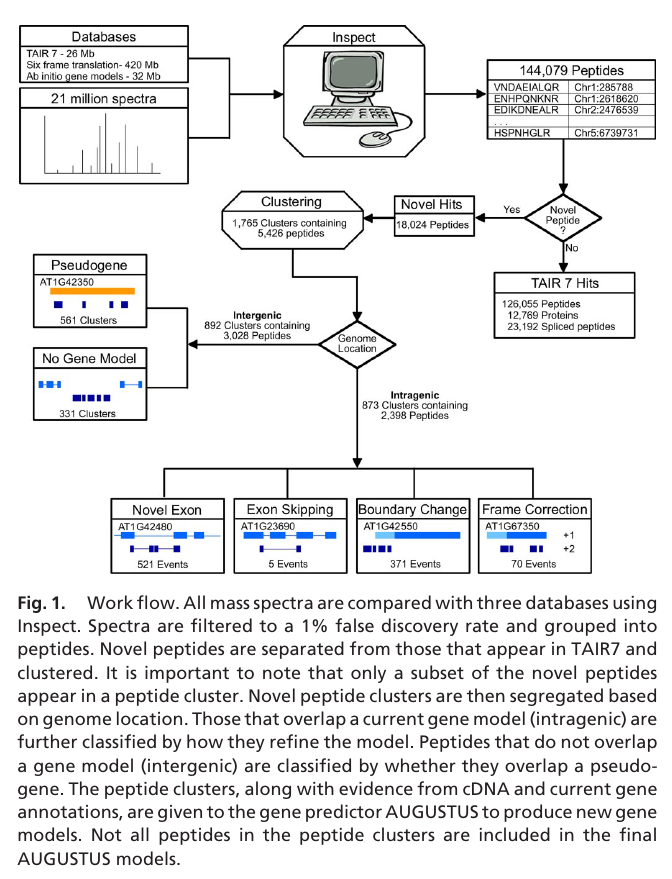
\includegraphics[width=0.5\textwidth]{castellana-2008-fig1}
        \caption{Castellana (2008) fig1}
    \end{figure}
    \FloatBarrier
